\subsection{Synthetic}\label{sec:synthetic_conversions}
\begin{figure}[H]
    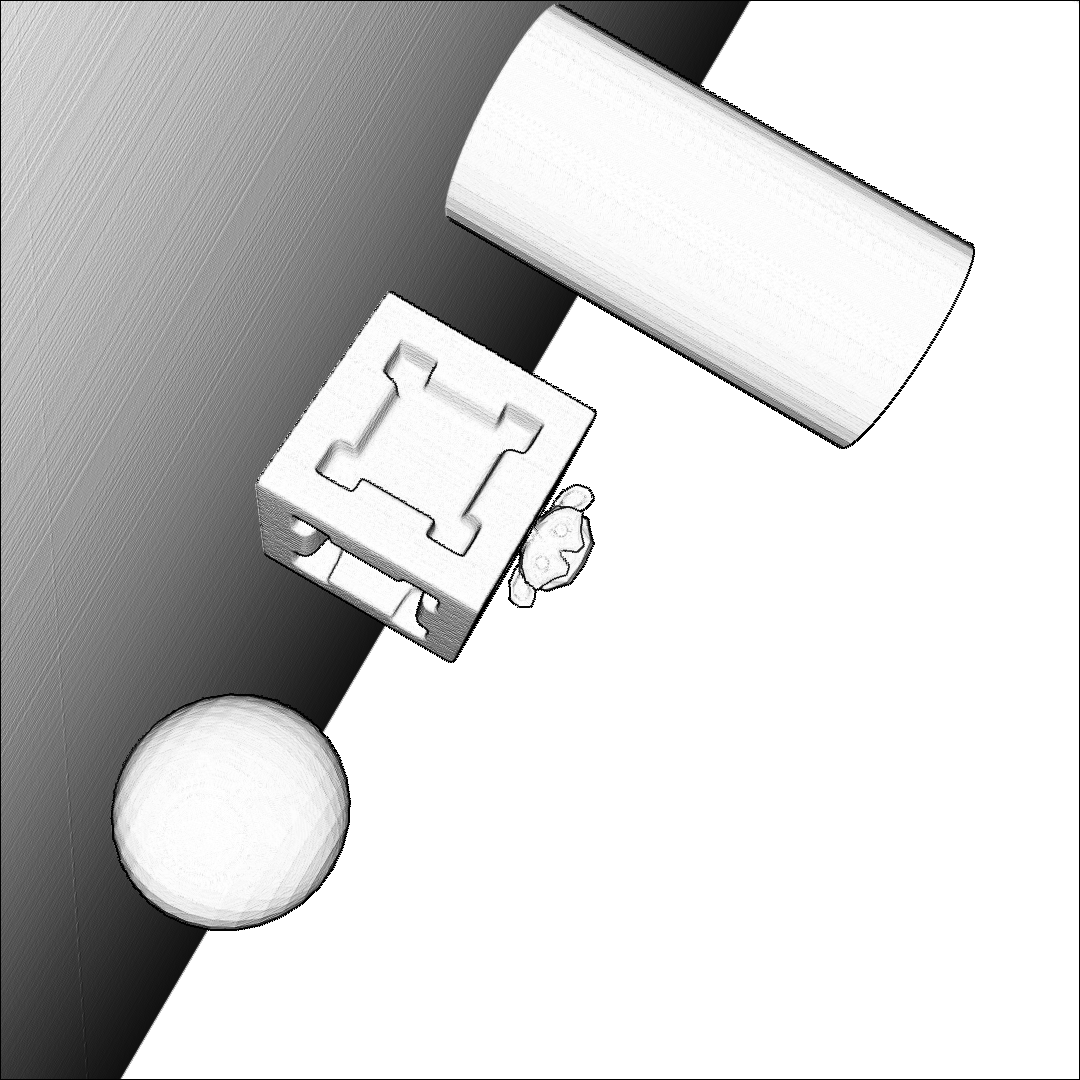
\includegraphics[width=0.25\linewidth]{chapter06/results/conv_images/synthetic/flexion/raw/0040.png}%
    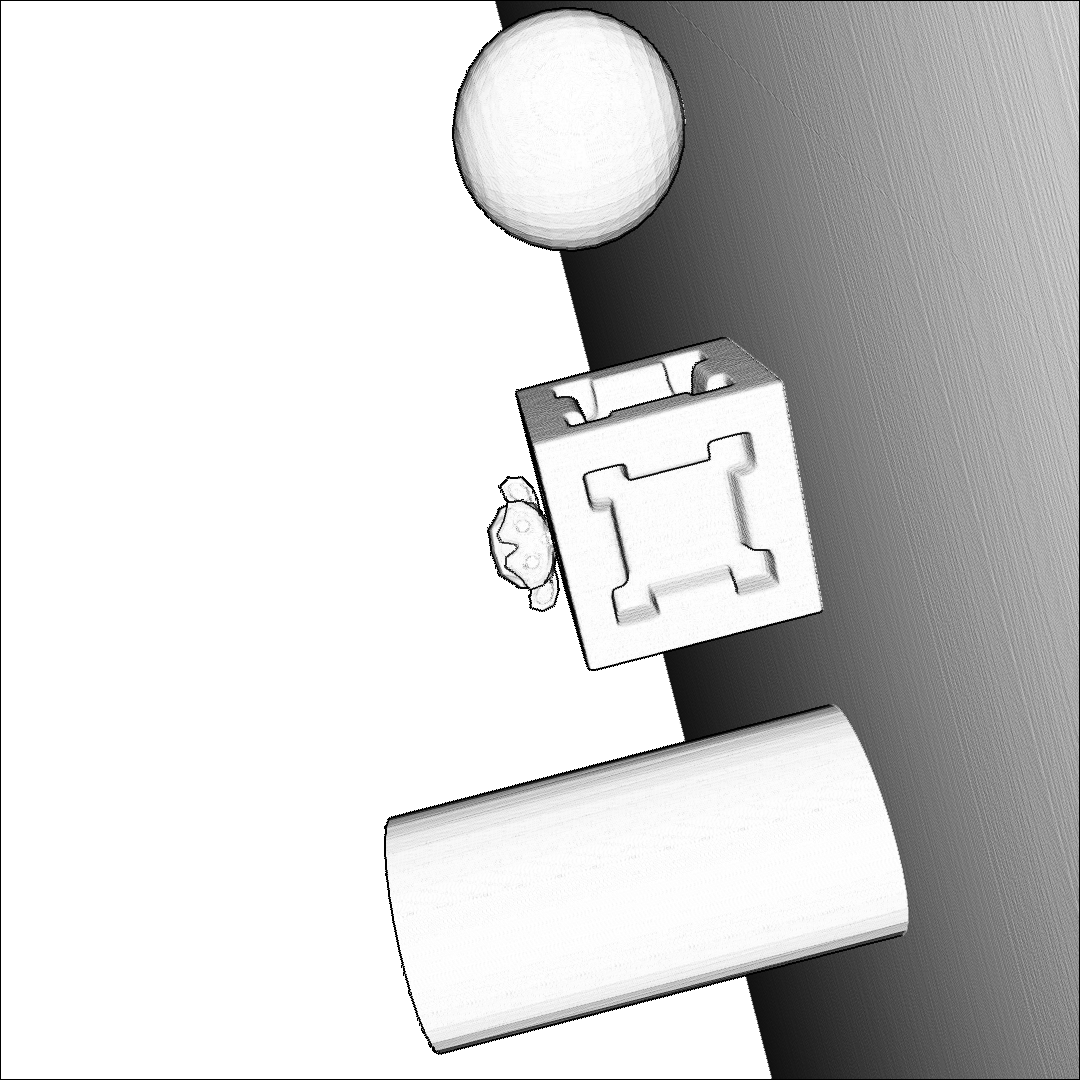
\includegraphics[width=0.25\linewidth]{chapter06/results/conv_images/synthetic/flexion/raw/0080.png}%
    
\includegraphics[width=0.25\linewidth]{chapter06/results/conv_images/synthetic/flexion/raw/0120.png}%
    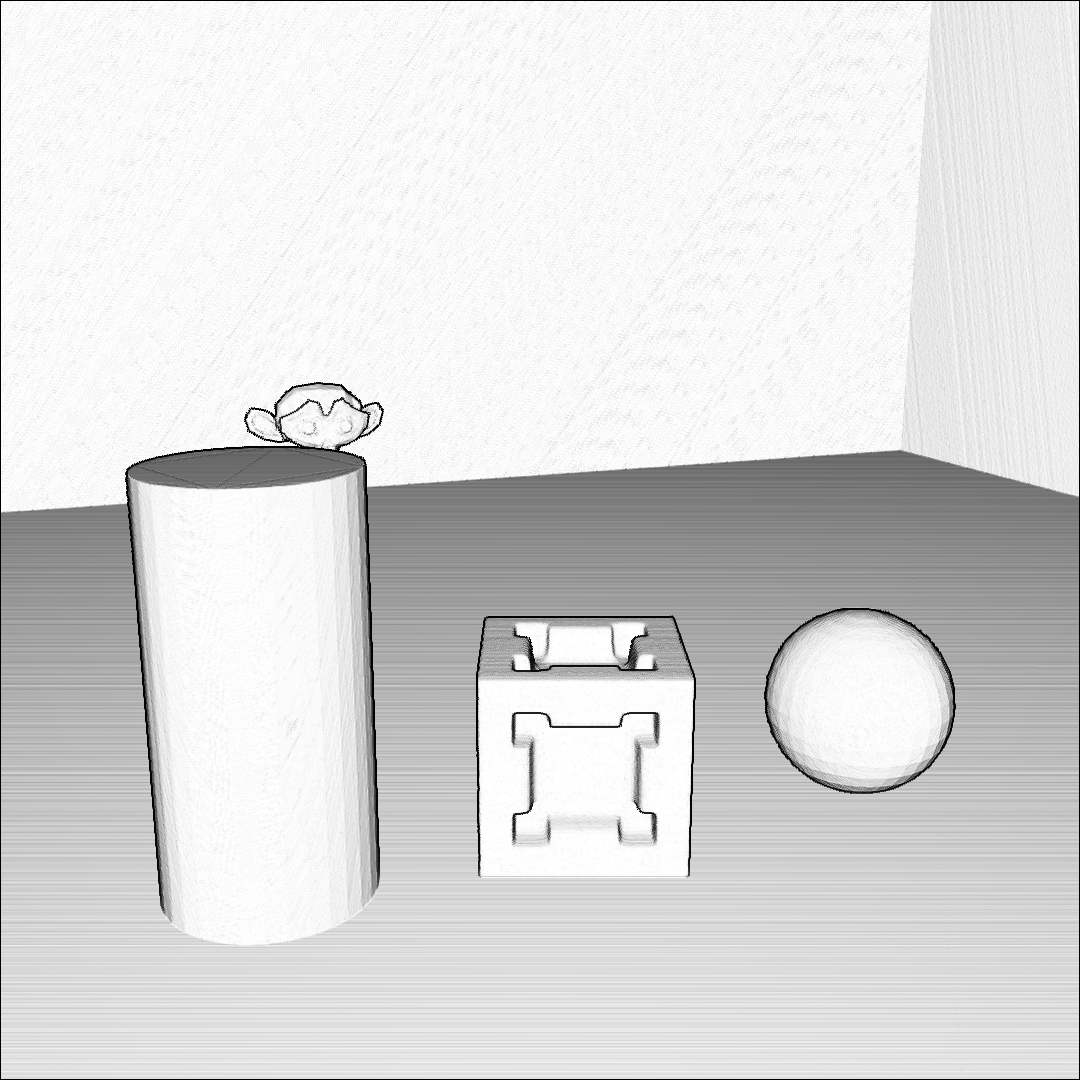
\includegraphics[width=0.25\linewidth]{chapter06/results/conv_images/synthetic/flexion/raw/0160.png}\\
    
\includegraphics[width=0.25\linewidth]{chapter06/results/conv_images/synthetic/bearing/raw/0040.png}%
    
\includegraphics[width=0.25\linewidth]{chapter06/results/conv_images/synthetic/bearing/raw/0080.png}%
    
\includegraphics[width=0.25\linewidth]{chapter06/results/conv_images/synthetic/bearing/raw/0120.png}%
    
\includegraphics[width=0.25\linewidth]{chapter06/results/conv_images/synthetic/bearing/raw/0160.png}%
    \caption[Examples of the \emph{Synthetic} scene feature image conversions]{\emph{Examples of the Synthetic scene feature image conversions.} The \emph{Synthetic} scene's conversion to \glspl{flexion-image} and \glspl{bearing-angle-image}. No filtering is applied, because the range data has no error.}
\end{figure}
